\titlepageframe % Specific command

% OBJETIVOS %

\begin{tframe}{Objetivos}
	\begin{itemize}
			\item Crear las bases, extendibles y genéricas, de un videojuego \textit{roguelike}
			\item Añadir elementos de accesibilidad, en especial para invidentes
	\end{itemize}
\end{tframe}

% QUÉ ES UN ROGUELIKE %

\begin{tframe}{Objetivos}
	\begin{itemize}
			\item<+-| alert@+> Crear las bases, extendibles y genéricas, de un videojuego \textit{roguelike}
			\item Añadir elementos de accesibilidad, en especial para invidentes
	\end{itemize}
\end{tframe}

\begin{tframe}{¿Qué es un \textit{roguelike}?}
	Género de videojuegos que suele contener los siguientes elementos:
	\begin{itemize}
		\item<+-| alert@+> Gran dificultad
			\begin{itemize}
				\item Muerte permanente o \textit{permadeath}
				\item Escalable en base al jugador
			\end{itemize}
	\end{itemize}
\end{tframe}

\begin{tframe}{¿Qué es un \textit{roguelike}?}
	Género de videojuegos que suele contener los siguientes elementos:
	\begin{itemize}
		\item Gran dificultad
			\begin{itemize}
				\item Muerte permanente o \textit{permadeath}
				\item Escalable en base al jugador
			\end{itemize}
		\item<+-| alert@+> Aleatoriedad
		\begin{itemize}
			\item Mapas
			\item Enemigos
			\item Objetos
		\end{itemize}
	\end{itemize}
\end{tframe}

\begin{tframe}{¿Qué es un \textit{roguelike}?}
	Género de videojuegos que suele contener los siguientes elementos:
	\begin{itemize}
		\item Gran dificultad
			\begin{itemize}
				\item Muerte permanente o \textit{permadeath}
				\item Escalable en base al jugador
			\end{itemize}
		\item Aleatoriedad
		\begin{itemize}
			\item Mapas
			\item Enemigos
			\item Objetos
		\end{itemize}
			\item<+-| alert@+> Exploración
	\end{itemize}
\end{tframe}

% Roguelike en nuestro proyecto %

\begin{tframe}{Elementos \textit{roguelike} en nuestro proyecto}
	En nuestro proyecto tenemos las siguientes características:
	\begin{itemize}
		\item<+-| alert@+> Gran dificultad
			\begin{itemize}
				\item Diferentes clases de enemigos que se adaptan al nivel del usuario
				\item Enemigos con distintas IAs
			\end{itemize}
	\end{itemize}
\end{tframe}

\begin{tframe}{Elementos \textit{roguelike} en nuestro proyecto}
	En nuestro proyecto tenemos las siguientes características:
	\begin{itemize}
		\item Gran dificultad
			\begin{itemize}
				\item Diferentes clases de enemigos que se adaptan al nivel del usuario
				\item Enemigos con distintas IAs
			\end{itemize}
		\item<+-| alert@+> Aleatoriedad
		\begin{itemize}
			\item Aleatoriedad en mapa y habitaciones
			\item Generador de encuentros: enemigos y objetos
		\end{itemize}
	\end{itemize}
\end{tframe}

% NO ES NADA DIFERENTE %

\begin{tframe}{Otros \textit{roguelikes} con las mismas ideas}
	FTL (Faster Than Light). 2012.
	\begin{figure}[h]
		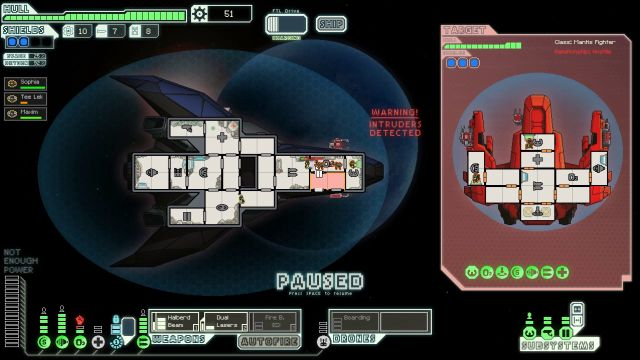
\includegraphics[width=8cm]{../img/ftl}
	\end{figure}
\end{tframe}

\begin{tframe}{Otros \textit{roguelikes} con las mismas ideas}
	Enter the gungeon. 2016.
	\begin{figure}[h]
		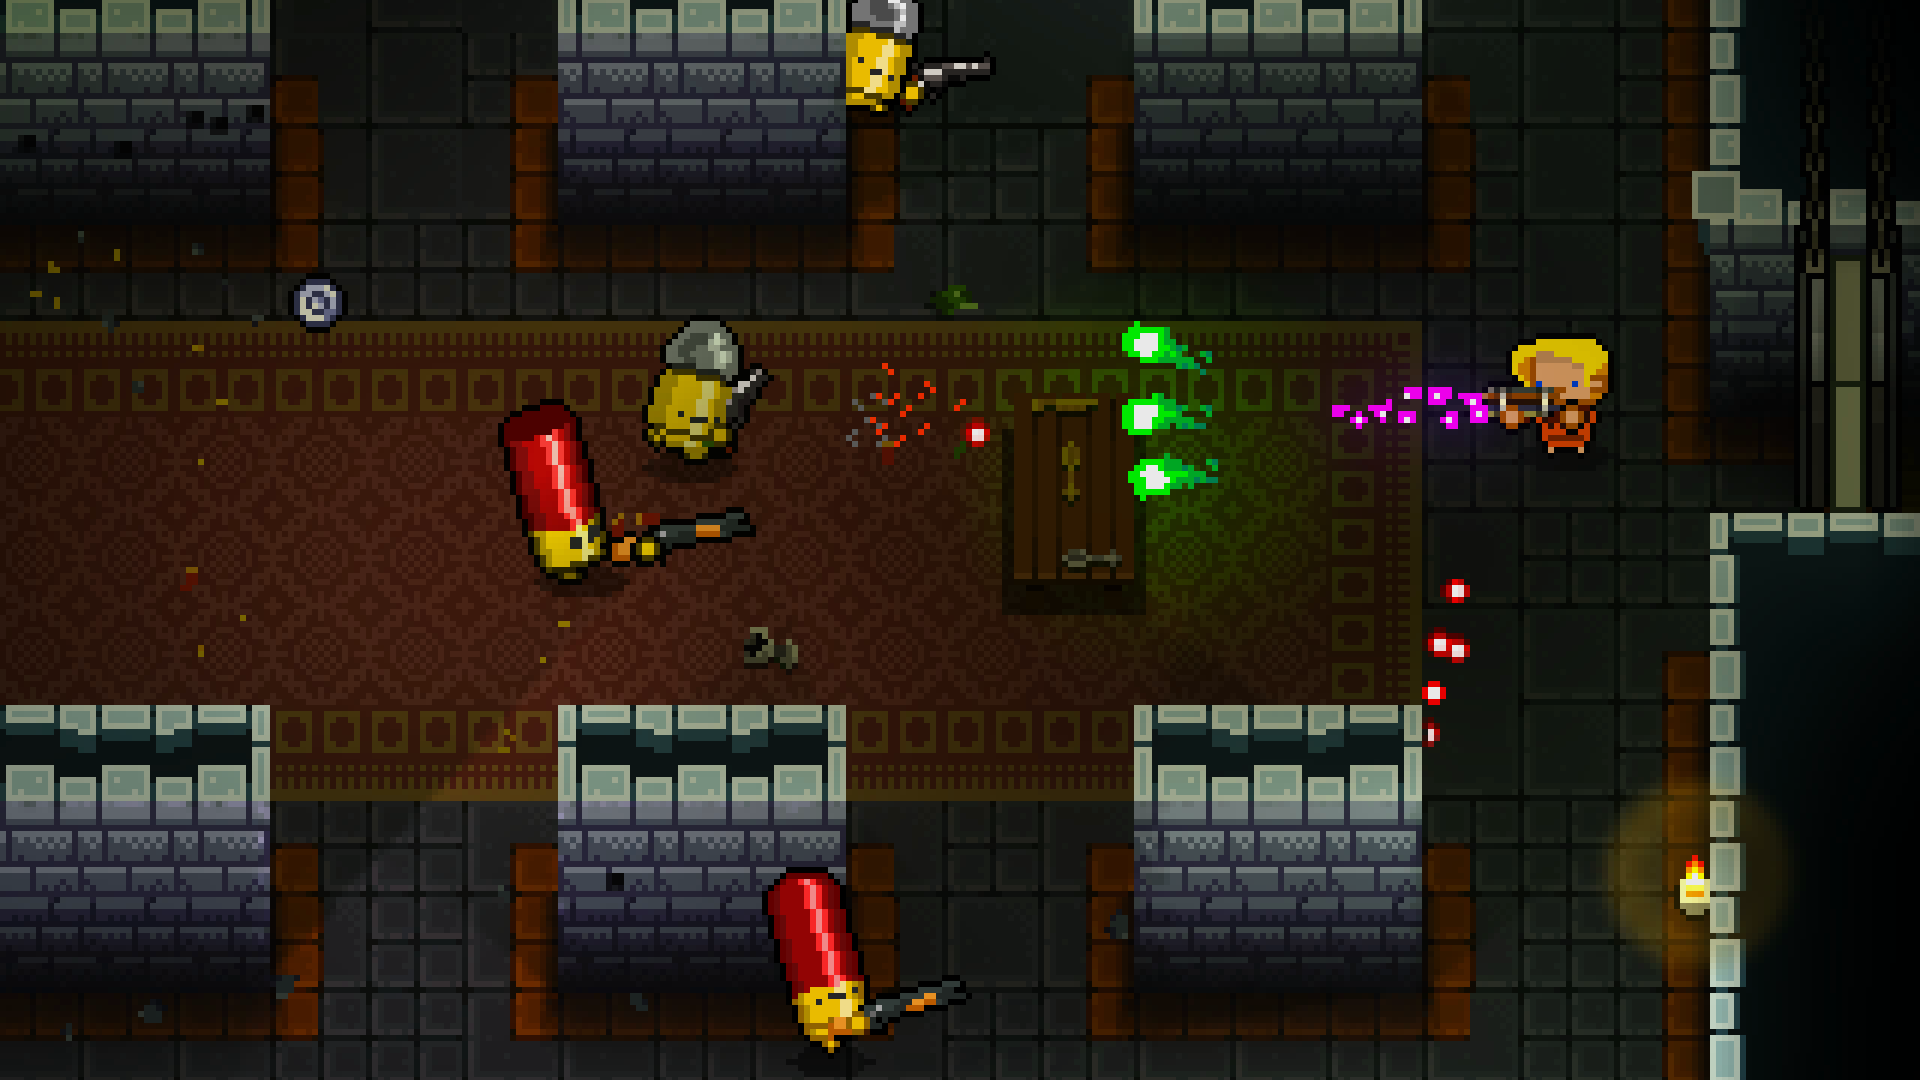
\includegraphics[width=8cm]{../img/enterthegungeon}
	\end{figure}
\end{tframe}

% POR QUÉ DISCRIMINAR? %

\begin{tframe}{Objetivos}
	\begin{itemize}
			\item Crear las bases, extendibles y genéricas, de un videojuego \textit{roguelike}
			\item<+-| alert@+> Añadir elementos de accesibilidad, en especial para invidentes
	\end{itemize}
\end{tframe}

\begin{tframe}{¿Por qué discriminar?}
	\begin{itemize}
			\item<+-| alert@+> Limitar el campo de visión (FOV)
	\end{itemize}
\end{tframe}

\begin{tframe}{¿Por qué discriminar?}
	\begin{itemize}
			\item Limitar el campo de visión (FOV)
			\item<+-| alert@+> No poder cambiar las teclas a usar
	\end{itemize}
\end{tframe}

\begin{tframe}{¿Por qué discriminar?}
	\begin{itemize}
			\item Limitar el campo de visión (FOV)
			\item No poder cambiar las teclas a usar
			\item<+-| alert@+> Obligar al jugador a distinguir colores para progresar
	\end{itemize}
\end{tframe}